\chapter{Level2 processor and I/O data}

\begin{figure}[t]
\centering
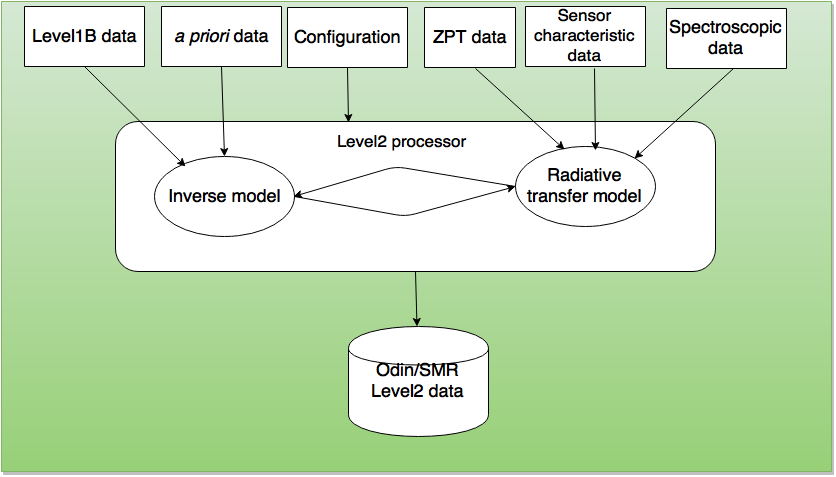
\includegraphics[width=14cm]{smr-level2-processor.png}
\caption{Schematic of the I/O data used and generated by the \smr\ Level2 processor.}
\label{fig:level2}
\end{figure}

\section{Level2 processor overview}

The \smr\ Level2 processor is designed to process
measurements from a scan of \smr\ in order to
retrieve profiles of atmospheric species.    
The Level2 processor is an optimal estimation method (OEM)
implementation, which combines measurement
information with Ancillary/Auxiliary data
and applies a forward model, and an iterative
scheme is used to find a best solution.   
The details of the algorithms within the
\smr\ Level2 processor is described in \smr\ Level2 ATBD.

\section{Level2 processor input data}

Figure~\ref{fig:level2} describes, on a high level, the input data used
by the Level2 processor and the generated output data.
\smr\ applies a number of different observation modes,
but the Level2 processor is identical for the various modes,
in terms of the high level workflow.

The Level2 processor obtains the input data through a hierarcical 
REST API, and the API is described in Sect.~\ref{sec:api}.
A high level description of the input data is described 
in the proceeding sections, and the detailed data formats
are described in Appendix~\ref{sec:dataformat}.


\subsection{Level1B data}
The most basic input data to the Level2 processor is the Level1B data,
i.e. geolocated and calibrated spectra from a scan of \smr.

\subsection{Climatological \textit{apriori} data}

Climatology data, covering all species of interest is required, as
the OEM implementation needs a starting estimate for each profile
to be retrieved. The climatology cover vertical, seasonal,
and latitudinal variations of each species and is based on data
from ?.

\subsection{ZPT data}
The Level2 processor requires external ZPT data (altitude, pressure, temperature) 
data. The ZPT data is extracted from the ERA-Interim dataset for the geolocation
of the scan. ERA-Interim is a global atmospheric reanalysis from 1979, and 
data is available throughout the Odin mission. 

\subsection{Sensor characteristic data}
The forward model simulation of the Level2 processor takes into account 
sensor characteristic data, i.e. the antenna angular response, 
sideband filtering, and frequency response of each spectrometer channel. 

\subsection{Spectroscopic data}
Spectroscopic data is basic input to the forward model of the Level2
processor.

\subsection{Configuration}
\smr\ applies a number of different observation modes,
and for each mode a different configuration is applied
of the Level2 processor...


\section{Level2 processor Output Data}
The output of the Level2 processor is retrieved
profiles of atmospheric species, error estimates,
and auxiliary data.
A high level description of the output data is described
in the proceeding sections, and the detailed data formats
are described in Appendix~\ref{sec:dataformat}.  

\subsection{Level2 data}
\subsection{Auxiliary data}

\section{API description and calls for input data}
\label{sec:api}

This section describes an API and the calls used to get data 
to the Level2 processing.
The data is accessed through a hierarcical REST API where deeper URIs return more
specific data.  All call URIs have a common root \url{rest_api/<version>}, which
has been omitted below for clarity.  All GET calls return JSON objects unless
otherwise noted. Key/value pairs are listed as name of the key
along with the type of the corresponding value within parantheses, followed
by a brief description of the contents.  
%See the sections on the different
%data sources for specifications on the structure of their respective JSON
%objects.

The URI hierachy is organized in the following way:
\begin{itemize}
    \item \url{freqmode/<date>/}: Returns object, which describes which frequency modes that were deployed the
    given date
    \begin{itemize}
        \url{freqmode/<date>/<backend>/<freqmode>/}: Returns object, which describes log data of the scans
        for the given date and deployed frequency mode
        \begin{itemize}
           \item \url{scan/<backend>/<freqmode>/<scanID>/}: Returns object that describes Level1B data for a given scan       
           \item \url{ptz/<date>/<backend>/<freqmode>/<scanID>/}: Returns object that describes ptz data for a given scan
           \item \url{apriori/<species>/<date>/<backend>/<freqmode>/<scanID>/}: Returns object that describes \textit{a priori} data for a given scan
        \end{itemize}  
    \end{itemize}
\end{itemize}
  


\subsection{\url{freqmode/<date>/}}
Method: \emph{GET}

Returns object, which describes which frequency modes that were deployed the
given date (YYYY-MM-DD), with the following attributes:
\begin{itemize}
    \item Info:

        A list of objects containing information about which
        frequency modes that were mesured this date. 
        Each object contains the following keys:

        \begin{itemize}
            \item Backend \emph{(String)}: The backend for the data
            \item FreqMode \emph{(Int)}: The frequency mode for the data
            \item NumScan \emph{(Int)}: The number of available scans
            \item URL \emph{(URI)}: A URI 
                for getting more specific of the available scans\\ 
                 (\url{freqmode/<date>/<backend>/<freqmode>/})
        \end{itemize}
\end{itemize}

\subsection{\url{freqmode/<date>/<backend>/<freqmode>/}}
Method: \emph{GET}

Returns object, which describes log data of the scans  
for the given date, backend, and freqmode,
with the following attributes:

\begin{itemize}
    \item Info:

        A list of objects that describes each scans
        with some log data.  
        Each object contains the following keys:

        \begin{itemize}
            \item AltEnd \emph{(float)}: Tangent point altitude ([\,m\,]) for last spectrum in scan
            \item AltStart \emph{(float)}:Tangent point altitude for first spectrum in scan
            \item DateTime \emph{(str)}: Mean UTC datetime (datetime(first) + datetime(last))/2 of scan
            \item FreqMode \emph{(Int)}: Deployed frequency mode
            \item LatEnd \emph{(float)}: Latitude of tangent point for last spectrum in scan
            \item LatStart \emph{(float)}: Latitude at tangent point for first spectrum in scan
            \item LonEnd \emph{(float)}: Longitude of tangent point for last spectrum in scan
            \item LonStart \emph{(float)}: Longitude at tangent point for first spectrum in scan
            \item MJDEnd \emph{(float)}: Modified julian date for last spectrum in scan
            \item MJDStart \emph{(float)}: Modified julian date for first spectrum in scan
            \item NumSpec \emph{(int)}: Number of atmospheric spectra in scan
            \item ScanID \emph{(int)}: Satellite time word identifier of scan
            \item SunZD \emph{(float)}: Mean solar zenith angle  (SunZD(first) + SunZD(last))/2 for scan
            \item URLS a list of key/value describing URIs containing
            more detailed data
            \begin{itemize} 
                \item URL-apriori-<species> \emph{(URI)}: 
                A URI for getting \textit{a priori} data of the scan\\
                (\url{apriori/<species>/<date>/<backend>/<freqmode>/<scanID>/})
                \item URL-ptz \emph{(URI)}: A URI for getting ptz data for the scan\\
                (\url{ptz/<date>/<backend>/<freqmode>/<scanID>/})
                \item URL-spectra \emph{(URI)}: A URI for getting Level1B spectra of the scan\\         
                (\url{scan/<backend>/<freqmode>/<scanID>/})        
            \end{itemize}
       \end{itemize}   
\end{itemize}

\subsection{\url{scan/<backend>/<freqmode>/<scanID>/}}
Method: \emph{GET}

\subsection{\url{ptz/<date>/<backend>/<freqmode>/<scanID>/}}
Method: \emph{GET}

Returns an object that describes the ptz data of the scan,
with the following attributes:

\begin{itemize}
    \item Pressure \emph{(array of doubles)}: Pressure vector ([\,Pa\,])
    \item Temperature \emph{(array of doubles)}: Temperature vector([\,K\,])
    \item Altitude \emph{(array of doubles)}:  Altitude vector([\,m\,])
    \item Latitude \emph{(double)}: Latitude of PTZ data
    \item Longitude \emph{(double)}: Longitude of PTZ data
    \item MJD \emph{(double)}: Modified Julian Date of PTZ data

\end{itemize}

\subsection{\url{apriori/<species>/<date>/<backend>/<freqmode>/<scanID>/}}
Method: \emph{GET}

Returns an object that describes the \textit{a priori} data of the scan,
with the following attributes:

\begin{itemize}
    \item Pressure \emph{(array of doubles)}: Pressure vector ([\,Pa\,])
    \item VMR \emph{(array of doubles)}: Climatology volume mixing ratio vector [\,--\,] of the species
    \item Species \emph{(String)}: description of species, i.e. one of 'BrO', 'Cl2O2', 'CO',
          'HCl', 'HO2', 'NO2', 'OCS', 'C2H2', 'ClO', 'H2CO', 'HCN', 'HOBr', 'NO', 'OH', 'C2H6',
          'ClONO2', 'H2O2', 'HCOOH', 'HOCl', 'O2', 'SF6', 'CH3Cl', 'ClOOCl', 'H2O', 'HF', 'N2', 'O3',
          'SO2','CH3CN', 'CO2', 'H2S', 'HI', 'N2O', 'OBrO', 'CH4', 'COF2', 'HBr', 'HNO3', 'NH3', or 'OClO'.
\end{itemize}



